\documentclass[letterpaper,10pt,conference]{ieeeconf}
\overrideIEEEmargins
\usepackage{amsmath,amssymb,graphicx,tabularx}
\usepackage{times}
\title{When Training Gets Easier: Range Collapse and Tracking Drift in Humanoid Robustness Training}
\author{Anonymous authors}
\begin{document}
\maketitle
\thispagestyle{empty}\pagestyle{empty}


\begin{abstract}

Robustness training can improve its dashboard while weakening the behavior it is intended to protect. We characterize two such failures in simulated humanoid motion tracking. First, an adaptive domain-randomization curriculum can increase return by narrowing its own training distribution. All six adaptive runs shrink their ranges; two nearly collapse. Across twelve evaluated runs, terminal return and independently measured robustness are inversely ranked (Spearman -0.73). A never-shrink projection blocks all 2,033 requested reductions across three seeds and satisfies a preregistered empirical tolerance rule against fixed randomization, without establishing statistical equivalence. Second, continued hard-condition training can retain 100\% nominal completion while degrading motion fidelity. In a one-origin, one-motion continuation study, nominal global pose error rises from 127.93 to 225.87 mm without anchoring. Reference-policy anchoring limits the endpoint increase to 4.33\%, passes the empirical retention checks at five sampled checkpoints, and improves hard-condition tracking-qualified execution by 5.18 percentage points over the origin. These are diagnostic and development findings, not evidence of curriculum superiority. Together they motivate evaluating training-distribution coverage and origin-relative tracking quality independently of return and survival.

\end{abstract}
\section{Introduction}

A humanoid can appear to improve for two different reasons that do not imply better task execution. Its training conditions can become easier, or its behavior can become more conservative while drifting away from the requested motion. Both changes can improve commonly monitored scores. Neither is visible from those scores alone.

We study these problems on a 29-DoF Unitree G1 motion-tracking task using SONIC. The first question is whether increasing training return reflects increasing robustness. In six long runs, a mismatch-driven adaptive randomization curriculum shrinks its physical ranges in every run and nearly collapses them in two. The collapsed runs have the highest terminal returns. On an independently fixed physics ladder, one loses 14.19 success-AUC points against fixed randomization on the same seed.

A monotonic projection closes this route to easier training: accept an expansion or hold the current range, but reject a reduction. It blocks every requested shrinkage across three seeds. The resulting policies pass a predefined empirical tolerance rule against fixed randomization. Their mean frontier difference is +0.60 points with sample standard deviation 2.25; the one-sided 95\% lower bound is -3.19 points, outside the 2-point margin. The evidence supports the recorded tolerance decision, not equivalence or a robustness advantage.

The second question is whether survival implies faithful motion execution. Starting from a solved local policy, hard-practice continuation preserves nominal completion while substantially increasing global pose error. Holding the practice mixture fixed does not prevent this loss. A reference-action penalty on cached origin states provides a useful protected baseline: at 2,000 iterations, its nominal global error is 133.47 mm against the origin's 127.93 mm, while an unanchored continuation reaches 225.87 mm. All three complete the nominal panel. Survival therefore cannot substitute for an independent retention measurement.

We make four bounded contributions:

\noindent 1. Measure training-range collapse and return--robustness inversion in a controlled humanoid curriculum study.\par
\noindent 2. Test a never-shrink rule that removes the observed range-contraction mechanism, with three-seed uncertainty and a strong fixed-randomization comparison.\par
\noindent 3. Demonstrate completion--fidelity decoupling during continuation and show that optimizer-history restoration alone does not explain it.\par
\noindent 4. Establish a reference-anchored fixed-practice development baseline that retains the tested motion within empirical budgets while improving hard-condition tracking qualification over its origin.\par

Monotonic projection and behavior regularization are established ideas, not stand-alone algorithmic novelty. The contribution is the measured failure chain, its controls, and the distinction between scores that appear favorable and the behaviors they fail to certify. Recovery-aware curricula remain future work and must outperform equally protected fixed training before receiving credit.

\section{Background and Related Work}

\textbf{Domain randomization} trains on a distribution of physical parameters so that the deployed system falls inside or near the training distribution [1--4]. \textbf{Adaptive randomization} changes that distribution during training. Automatic Domain Randomization expands boundaries after performance at the boundary passes a threshold [5]; active and entropy-based methods choose which domains to sample [6,7]; self-paced and teacher-based curricula trade difficulty against learning progress [8,9]; level-replay methods emphasize informative levels [14,15]. Several of these methods are allowed to make training easier when the policy struggles. That freedom is the subject of this paper.

The never-shrink rule we test is close to the boundary rule in Automatic Domain Randomization. We do not claim it as new. Our contribution is the measurement of what goes wrong without it in long humanoid runs, the empirical comparison against fixed randomization, and the limits of the readiness signals used to drive expansion.

\textbf{Humanoid motion tracking.} DeepMimic, adversarial motion priors, BeyondMimic, and SONIC learn reference-conditioned whole-body control [10--13]. We use SONIC as the sole testbed. It provides a 29-DoF Unitree G1 model, a 50 Hz policy, Isaac Lab training, and a MuJoCo model.

\textbf{Evaluation beyond reward.} Training return depends on the distribution it is measured on. We therefore score every policy on a frozen physics ladder that the curriculum never sees, and report success and restricted-mean progress rather than reward [19].

Reference behavior can also be protected during fine-tuning. PPF regularizes toward a model-based controller where its assumptions remain reliable [20]; our cached-origin action penalty is a different implementation of behavior preservation, not a claim to invent it. DORAEMON [7] already constrains randomization expansion by performance. A future quality-aware curriculum must therefore establish an advantage beyond a protected fixed baseline, rather than attributing anchoring or a stricter success definition to curriculum feedback.

\section{Setup}

\textbf{Task.} A policy tracks one reference clip (\texttt{walk\_hands\_on\_back\_loop\_002}, 4 s) on a
29-DoF G1 in Isaac Lab, 1,024 parallel environments, 8,000 PPO iterations, trained from scratch. The actor sees a ten-step history of gravity direction, base angular velocity, joint positions, joint velocities, and previous actions, plus ten future reference frames.

\textbf{Randomized parameters.} Six channels: rigid-body mass, torso center of mass, joint default offset, ground friction, action delay, and external pushes. A scale $\lambda$ multiplies every channel's configured deviation; $\lambda$ = 1 is the training envelope and $\lambda$ = 0 is nominal physics. Friction is clipped at a physical floor, which binds at $\lambda$ $\geq$ 1.5.

\textbf{Compared training arms.}

\begin{table}[t]\small
\begin{tabularx}{\linewidth}{XX}\hline
Arm & Training ranges \\\hline
No randomization & $\lambda$ = 0 throughout \\
Fixed randomization & $\lambda$ = 1 throughout \\
Adaptive, may shrink & $\lambda$ set by a PI controller on a learned mismatch signal, $\lambda$ $\in$ [0, 1] \\
Adaptive, never shrinks & same controller, but a requested decrease is refused \\
\hline\end{tabularx}\end{table}

Two variants of the adaptive controller and three seeds give the six adaptive runs.

\textbf{Evaluation.} Each final policy is scored on a frozen ladder of physics scales
\{0, 0.25, 0.5, 0.75, 1, 1.25, 1.5, 1.75, 2\} with 512 episodes per cell. The primary outcome is the area under the success-versus-scale curve over the beyond-envelope cells (\textbf{frontier AUC}, reported in points, 0--100) and over the in-envelope cells. Restricted-mean progress is a secondary outcome. The ladder is never visible to any curriculum.

\section{The Problem: Training-Range Collapse}
\begin{figure}[t]\centering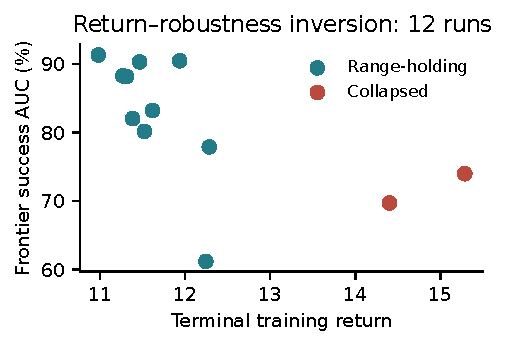
\includegraphics[width=\linewidth]{figures/return_inversion.pdf}\caption{Terminal return versus frontier success AUC for twelve historical runs. Each point is one trained policy; the two collapsed runs have the highest returns. Descriptive Spearman correlation: -0.73.}\end{figure}

\subsection{A conditional contraction mechanism}

Let the curriculum observe a score $\bar Y(\theta,\lambda)$ on its own training distribution and move $\lambda$ toward a set point $Y^*$ with an integral rule $\dot\lambda = K(\bar Y - Y^*)$. Wider ranges lower the score, $\partial \bar Y/\partial\lambda < 0$. When learning stalls and the score sits below the set point, the controller lowers $\lambda$, which raises the score without any change in the policy. If the policy adapts to hard physics more slowly than the controller moves $\lambda$, shrinking is the fast response of the coupled system, and the gain $K$ sets the speed of collapse rather than its direction. This is a conditional statement about one common controller form, not a theorem about every adaptive curriculum; a deadband, saturation, or policy recovery can interrupt it. It says where to look.

\subsection{What we observed}

Every one of the six adaptive runs applied at least one reduction. Two ended near $\lambda$ = 0 after having reached the full envelope earlier in training.


\begin{table*}[t]\small
\textbf{Table 1. Collapsed runs against the runs that held their ranges.}\par\medskip
\begin{tabularx}{\linewidth}{XXXX}\hline
Outcome & Collapsed run A & Collapsed run B & Range-holding runs (min--max) \\\hline
Final scale $\lambda$ & 0.062 & 0.012 & 1.000 \\
Mean return, last 500 iterations & \textbf{15.29} & \textbf{14.40} & 10.98--12.28 \\
Frontier success AUC (points) & 73.99 & 69.73 & 61.20--91.31 \\
\hline\end{tabularx}\end{table*}

The collapsed runs have the two highest terminal returns among the twelve arm--seed pairs we scored. Across the twelve, terminal return and frontier AUC have Spearman rank correlation
-0.73: the runs that look best from inside training are the ones that retreated furthest from the deployment physics. Grouped, the collapsed runs average return 14.84 and AUC 71.9; the range-holding runs average return 11.60 and AUC 83.3.

\textbf{Cost.} Collapsed run A was chosen for scoring before its evaluation existed. It scores
14.19 points below fixed randomization on the same seed and 17.32 points below the never-shrink version of the same controller on the same seed.

This differs from ordinary forgetting. Forgetting means later training damages an earlier skill. Collapse means the curriculum removes the conditions that would reveal the damage and then grades itself on the easier replacement.

\section{A Rule That Prevents Shrinkage}
\begin{figure}[t]\centering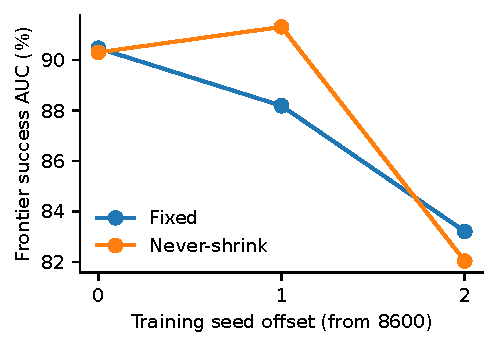
\includegraphics[width=\linewidth]{figures/paired_seeds.pdf}\caption{Three paired training seeds. The never-shrink versus fixed difference averages +0.60 points (SD 2.25); the empirical tolerance pass does not establish equivalence.}\end{figure}

We keep the same controller and refuse every requested decrease. The range may expand or hold; it may not shrink: $\lambda_{n+1}=\max(\lambda_n,\widetilde\lambda_{n+1})$, where the tilde denotes the unchanged controller proposal.

\textbf{Mechanism.} Across three seeds the rule refused 453, 951, and 629 requested reductions,
2,033 in total, and applied none. All three runs ended at the full envelope. These requests are correlated controller events, not independent samples; their role is to show sustained pressure toward easier training across the long runs. The sample size for any policy comparison is three seeds.

\textbf{Robustness.} The comparison follows a rule fixed before the data: for each of four AUC components the never-shrink arm must be within 2 points (frontier) or 1 point (in-envelope) of fixed randomization on at least two of three paired seeds.


\begin{table*}[t]\small
\textbf{Table 2. Never-shrink versus fixed randomization, frontier success AUC (points).}\par\medskip
\begin{tabularx}{\linewidth}{XXXX}\hline
Seed & Never-shrink & Fixed & Difference \\\hline
8600 & 90.30 & 90.46 & -0.16 \\
8601 & 91.31 & 88.18 & +3.13 \\
8602 & 82.03 & 83.20 & -1.17 \\
\textbf{Mean} &  &  & \textbf{+0.60} (SD 2.25) \\
\hline\end{tabularx}\end{table*}

All four components pass on all three seeds (frontier success +0.60, in-envelope success
+0.07, frontier progress +0.50, in-envelope progress +0.01). Two seeds favour fixed randomization slightly.

\textbf{What that does and does not establish.} The rule was fixed before the data and it passed; that is the decision it was written to make. It is not a demonstration of equivalence. With three seeds and a paired standard deviation of 2.25 points, the one-sided 95\% lower bound on the frontier-success difference is -3.19 points, which lies outside the 2-point margin. A proper equivalence claim needs enough seeds for the interval to sit inside the margin, and we do not have them. The supported statement is narrower: the predefined empirical tolerance rule passed, while an advantage or a statistical noninferiority claim remains unsupported. Retaining the ranges also does not by itself guarantee that the policy retains its skills; Table 2 measures robustness, while Section 8 separately tests tracking retention.

\textbf{Realized exposure.} Training telemetry records how many episodes each training cohort ran and at what intensity, so realized practice can be counted rather than assumed. The never-shrink arm spent 99.2 percent of its training exposure at the envelope, against 100 percent for fixed randomization. Their realized intensity exposure is very similar. This is consistent with their similar outcomes, but does not establish identical trajectories or a causal explanation.

\textbf{Seed effect.} Between-seed offsets in frontier AUC reach 7.8 points on the same arm. Any claimed advantage of a curriculum over fixed randomization must be paired by seed and must clear this before it is believed.

\section{Which Signals Can Guide Expansion}
\begin{figure}[t]\centering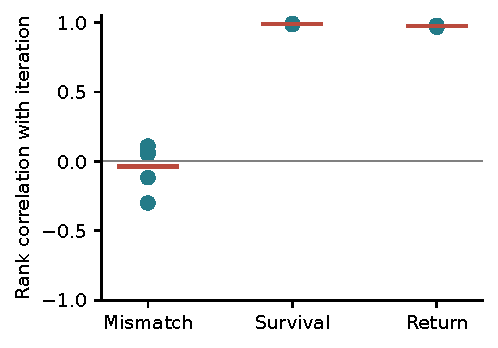
\includegraphics[width=\linewidth]{figures/signal_audit.pdf}\caption{Fixed-difficulty signal audit. Dots are run-level rank correlations with iteration; horizontal marks are their means. Correlation with progress is not a recovery or fidelity guarantee.}\end{figure}

A signal that drives an expanding curriculum must move with competence when difficulty is fixed, and must respond to difficulty in the right direction. We audited five signals on five runs at pinned difficulty and on the two collapses.


\begin{table*}[t]\small
\textbf{Table 3. Readiness-signal audit.}\par\medskip
\begin{tabularx}{\linewidth}{XXXXX}\hline
Signal & Rank correlation with training iteration at fixed $\lambda$ & Direction reversals & Behaviour during the two collapses & Use \\\hline
Time-out survival & +0.987 & 4.6 & rises when ranges shrink & readiness signal, but only if measured on proposed conditions \\
Mean return & +0.973 & 3.2 & rewards shrinking strongly & diagnostic only \\
Learned mismatch & -0.037 & 19.2 & -0.03 / +0.03 against $\lambda$ & rejected \\
Foot slip per step & -0.531 & 17.0 & +0.75 / +0.71 against $\lambda$ & corroborating measurement \\
Torque saturation & -0.312 & 7.2 & sign flips across arms & cost, not a gate \\
\hline\end{tabularx}\end{table*}

The learned mismatch signal fails these empirical competence and difficulty checks. That is consistent with its poor suitability for the tested controller, but does not isolate a causal explanation for collapse. Survival is a stronger competence correlate in this audit; evaluating it only on a shrinking training distribution can still inflate it. Even an independent survival probe cannot certify fidelity, as Section 8 demonstrates.

\section{Robustness Is Per-Parameter and Interactive}

We widened one channel at a time on frozen policies, holding the others at the envelope,
512 episodes per cell, one seed.


\begin{table*}[t]\small
\textbf{Table 4. Success when one channel is widened beyond its training range.}\par\medskip
\begin{tabularx}{\linewidth}{XXXXXXX}\hline
Policy & All channels 2$\times$ & Mass 2$\times$ / 3$\times$ & Center of mass 2$\times$ / 3$\times$ & Joint offset 2$\times$ / 3$\times$ & Push 2$\times$ / 3$\times$ & First to fail \\\hline
Fixed & 0.820 & 0.992 / 0.949 & 0.988 / 0.988 & 0.992 / 0.990 & \textbf{0.912 / 0.746} & push \\
Never-shrink & 0.842 & 0.990 / 0.938 & 0.992 / 0.982 & 0.994 / 0.986 & \textbf{0.928 / 0.770} & push \\
Adaptive, held ranges & 0.795 & 0.980 / 0.951 & 0.986 / 0.975 & 0.994 / 0.980 & \textbf{0.910 / 0.705} & push \\
Adaptive, collapsed & 0.518 & 0.873 / 0.682 & 0.928 / 0.818 & 0.967 / 0.955 & \textbf{0.811 / 0.570} & push \\
No randomization & 0.334 & 0.795 / 0.643 & \textbf{0.654 / 0.393} & 0.900 / 0.891 & 0.736 / 0.443 & center of mass \\
\hline\end{tabularx}\end{table*}

For the three healthy policies, pushes at twice the range cost 6--8 points while mass, center of mass, and joint offsets cost at most 1.4 points and stay above 0.938 at three times the range. The unrandomized policy fails first under center-of-mass shift instead. Which parameter binds depends on the policy, so it must be measured for the policy being trained rather than assumed from the simulator.

Widening everything together costs more than the parts. For the fixed policy the individual
2$\times$ losses sum to 0.111 while the joint 2$\times$ cell loses 0.174, about six points that no sum of single-channel losses predicts. The joint cell widens five channels at once, so we do not attribute the residual to any pair; a pairwise sweep is the test.

\section{Survival Is Not Fidelity}
\begin{figure*}[t]\centering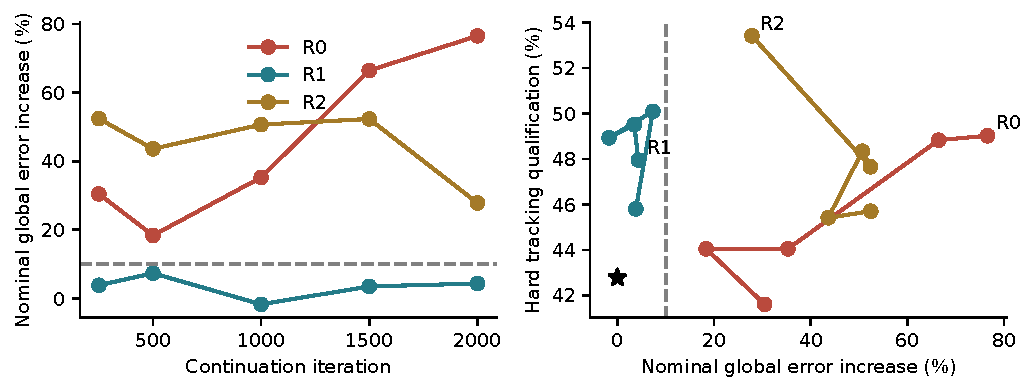
\includegraphics[width=\linewidth]{figures/retention_trajectory.pdf}\caption{One-origin, one-motion development continuation. Left: nominal global-error trajectories. Right: hard tracking qualification versus nominal error increase. Dashed lines mark the empirical 10 percent nominal budget only; the full retention gate also checks local error and original-envelope conditions. Each point uses 512 aliases per condition; trajectories are not independent training replicates.}\end{figure*}

\subsection{Origin-relative measurement}

Range preservation and behavior preservation are separate requirements. In an earlier quality-frontier pilot, a survival-feedback gate retains 100\% nominal completion while the legacy evaluation panel's global MPJPE rises from 128.57 to 324.50 mm (+152.39\%). At the shared Push 3.5$\times$ condition, completion increases from 64.84\% to 71.09\%, but tracking-qualified execution decreases from 49.02\% to 45.70\%. The latter requires completion and episode-mean global/local errors below 600/50 mm. These deliberately broad development thresholds do not certify high-quality imitation or return-to-path recovery.

The initial gate passed checks relative to other continued policies, yet all continued policies had degraded. Comparisons among degraded controls cannot establish preservation of the starting skill. We therefore evaluate retained conditions against the same frozen origin. The later retention screen uses masked first-episode measurements and its own origin evaluation (127.93 mm); we do not combine that denominator with the earlier legacy panel.

Global and local pose errors are reported separately. Global MPJPE can reflect persistent root displacement as well as articulation and heading error; these scalar norms do not admit a simple additive translation-plus-local-error identity. The present data demonstrates tracking drift without identifying a unique physical compensation or proving intentional \texttt{}cheating.''

\subsection{Continuation controls}

Drift persists when the initial hard-practice mixture is held fixed. A separate fresh-versus-restored optimizer-history experiment also finds degradation in both branches. Thus neither expansion nor restoration of optimizer buffers is necessary for the observed loss. These controls do not identify the PPO objective as its unique cause: reward weighting, optimization dynamics, and changed visitation remain possible contributors.

We retain the selected fresh-optimizer recipe and compare three continuations from the same solved local origin. R0 uses unanchored fixed practice. R1 adds reference-action anchoring. R2 reduces the initial learning rate and keeps it fixed. R0/R1 start at $2\times10^{-5}$ with adaptive inner PPO learning-rate bounds $[10^{-5},2\times10^{-4}]$; R2 stays at $10^{-5}$. R2 changes the learning-rate schedule as well as its starting value, so it is not a pure learning-rate-magnitude ablation.

\subsection{A protected fixed-practice baseline}

All three arms use 1,024 environments, 2,000 PPO iterations, and the same 3:1 mixture of original-envelope and Push 3$\times$ practice. R1 adds a squared action-mean penalty on cached actor inputs and teacher targets from the origin, with coefficient 1 and batches of 256. The original observation and normalization contract is preserved. The penalty averages the summed squared differences over the batch, $\mathcal L_{\rm anchor}=B^{-1}\sum_{b=1}^{B}\|\mu_\theta(h_b)-\mu_0(h_b)\|_2^2$, in native pre-actuator action units (identity coordinate scaling); it is not averaged over action coordinates. Hard recovery states are not added to this nominal anchor buffer.

Retention requires global and local episode-mean errors to increase by at most 10\%, and completion to fall by at most two percentage points, separately under nominal and original-envelope conditions. We check iterations 250, 500, 1,000, 1,500, and 2,000 using 512 evaluation aliases per cell. These are empirical development gates, not simultaneous confidence guarantees.


\begin{table*}[t]\small
\textbf{Table 5. Continuation endpoints. Hard qualification equally averages Push 3.5$\times$ and Push 3.5$\times$ plus friction 1.5$\times$.}\par\medskip
\begin{tabularx}{\linewidth}{XXXXX}\hline
Policy & Nominal global / local MPJPE (mm) & Global increase & Hard qualification & All five retention gates \\\hline
Origin & 127.93 / 28.19 & Reference & 42.77\% & Reference \\
R0 & 225.87 / 30.21 & +76.56\% & 49.02\% & Fail \\
R1 & 133.47 / 27.96 & +4.33\% & 47.95\% & Pass \\
R2 & 163.53 / 28.31 & +27.83\% & 53.42\% & Fail \\
\hline\end{tabularx}\end{table*}

Every endpoint completes the nominal panel at 100\%. R1 alone satisfies all sampled retention gates. Its hard-qualified score improves by 5.18 percentage points over origin, while R0 and R2 obtain larger unconstrained gains but violate retention. The 4.33\% increase is R1's endpoint value, not its value at every checkpoint. R1 provides a feasible development tradeoff, not dominance on every metric or evidence that feedback schedules work.

Each arm receives 49,152,000 simulator transitions. R1 additionally uses 40,000 anchor updates, 10,240,000 anchor sample presentations, and 80,000 student forwards, with 207.37 seconds measured inside those forwards. Transitions are matched; total computation is not. One origin, one motion, and one continuation seed support this result. Hundreds of rollout aliases do not create independent training replicates.

\section{Does the Ordering Survive a Change of Simulator and Motion?}
\begin{figure}[t]\centering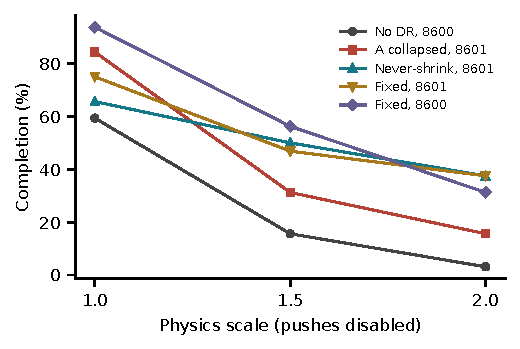
\includegraphics[width=\linewidth]{figures/mujoco_ladder.pdf}\caption{Historical exported policies in independently randomized MuJoCo, without pushes. Each point is a pass count over 32 physics draws; these are not 32 training seeds. At scale 2, paired fixed and never-shrink each pass 12/32, collapsed 5/32, and no DR 1/32. These are not the R1 checkpoints.}\end{figure}

\textbf{Second simulator.} We exported the final policies to ONNX and replayed them in MuJoCo with our own implementation of the six channels, scaled by the same $\lambda$. This is a sim-to-sim check of the exported policy, not the hardware deployment path, and MuJoCo's randomization is a labelled approximation of Isaac's. A run passes if the pelvis stays within 0.5 m of the reference to the end of the clip. Seeds are shared across arms, 32 per cell.


\begin{table}[t]\small
\textbf{Table 6. MuJoCo survival of exported policies (pass rate over 32 physics draws).}\par\medskip
\begin{tabularx}{\linewidth}{XXX}\hline
Policy & All channels, $\lambda$ 1 / 1.5 / 2 & Physics only (no pushes), $\lambda$ 1 / 1.5 / 2 \\\hline
No randomization & 31 / 12 / 0 \% & 59 / 16 / 3 \% \\
Adaptive, collapsed (seed 8601) & 56 / 19 / 9 \% & 84 / 31 / 16 \% \\
Never-shrink (seed 8601) & 47 / 22 / 16 \% & 66 / 50 / 38 \% \\
Fixed (seed 8601, paired) & 47 / 25 / 12 \% & 75 / 47 / 38 \% \\
Fixed (seed 8600) & 78 / 34 / 16 \% & 94 / 56 / 31 \% \\
\hline\end{tabularx}\end{table}

Pushes are the binding channel in MuJoCo as in Isaac, and absolute survival is far below the Isaac scores because the randomization differs; the gap is reported, not tuned. The ordering is what transfers. Beyond the training envelope without pushes, the never-shrink and paired fixed policies tie at 38\%, the collapsed policy reaches 16\%, and the unrandomized policy 3\%. Between the two seeds of fixed randomization the difference is as large as between methods, which repeats the seed effect of Section 5. These replays evaluate the historical range-control policies, not R1 or the future recovery-aware controller.

\textbf{Second motion.} On an untrained clip of the same family (\texttt{walk\_hands\_on\_back\_loop\_003},
128 episodes per cell), success at $\lambda$ 1.5 is 0.80 for fixed, 0.73 for the range-holding adaptive run, 0.40 for the collapsed run, and 0.18 without randomization. Rank correlation of the arm ordering with the trained clip is 0.8 and 1.0 across the two cells. This is one nearby clip, not motion generalization.

\section{Interpretation and Limits}

For a continuously uniform scalar parameter whose range scales affinely around its nominal value, the interval at intensity s has s times the width of the full interval. A full-intensity draw lands inside it with probability s and, conditional on doing so, has the same scalar distribution. Fixed randomization therefore withholds no marginal parameter values that an earlier nested stage would introduce. This is a support statement, not proof that fixed practice samples equally easy whole episodes or makes scheduling unnecessary. Discrete, clamped, and event-time implementations require their own treatment; joint difficulty and realized exposure are distinct from marginal support.

The historical practice-allocation, effort, and thermal-barrier screens did not establish an adaptive advantage. A progress-signal audit also found insufficient reliable online signal at the tested sampling budget. These null results bound the present evidence; neither nesting nor a negative audit proves that all curricula must fail. The same total budget can still be allocated differently in time, across motions, or across combinations. Any future feedback claim requires comparison with fixed and frozen schedules that share the same retention mechanism, allowed conditions, and resource accounting.

The range-control comparison has three seeds. Its empirical tolerance decision is weaker than demonstrated noninferiority, and the channel sweep has one seed. The continuation study has one local origin and one solved walking motion. Three longer development candidates were not qualified by that origin, so preserving a broader repertoire cannot be inferred. A nearby clip and an independently implemented MuJoCo replay provide limited transfer evidence for the historical policies only. Nothing here has been tested on hardware.

Global MPJPE does not identify a recovery process. A robot can finish a clip while displaced from its path; local articulation can remain good in that state. Recovery would require calibrated component thresholds, event timing, a dwell interval, and a sufficiently long observation window, together with controller inputs that identify the required correction. A separate released-controller and path-input programme addresses these prerequisites, but contributes no recovery efficacy claim here.

\section{Conclusion}

A robustness-training dashboard can hide two losses: the curriculum can narrow the conditions being practiced, and the policy can retain survival while losing motion fidelity. Independent evaluation exposes both in this humanoid testbed. A never-shrink projection blocks the observed contraction requests and passes a predefined empirical tolerance rule against fixed randomization. Reference anchoring provides a protected fixed-practice development result, limiting nominal drift while improving hard-condition tracking qualification over the origin. These findings motivate separate coverage and retention checks. They do not establish adaptive curriculum superiority, multi-motion preservation, or recovery after disturbance.

\section*{References}\small

\noindent [1] J. Tobin et al., "Domain Randomization for Transferring Deep Neural Networks from Simulation to the Real World," IROS, 2017.\par\medskip
\noindent [2] X. B. Peng et al., "Sim-to-Real Transfer of Robotic Control with Dynamics Randomization," ICRA, 2018.\par\medskip
\noindent [3] J. Tan et al., "Sim-to-Real: Learning Agile Locomotion for Quadruped Robots," RSS, 2018.\par\medskip
\noindent [4] A. Rajeswaran et al., "EPOpt: Learning Robust Neural Network Policies Using Model Ensembles," 2016.\par\medskip
\noindent [5] OpenAI et al., "Solving Rubik's Cube with a Robot Hand," 2019.\par\medskip
\noindent [6] B. Mehta et al., "Active Domain Randomization," CoRL, 2019.\par\medskip
\noindent [7] G. Tiboni et al., "Domain Randomization via Entropy Maximization," ICLR, 2024.\par\medskip
\noindent [8] P. Klink et al., "Self-Paced Contextual Reinforcement Learning," CoRL, 2020.\par\medskip
\noindent [9] R. Portelas et al., "Teacher Algorithms for Curriculum Learning of Deep RL in Continuously Parameterized Environments," CoRL, 2020.\par\medskip
\noindent [10] X. B. Peng et al., "DeepMimic," 2018.\par\medskip
\noindent [11] X. B. Peng et al., "AMP: Adversarial Motion Priors," 2021.\par\medskip
\noindent [12] Z. Luo et al., "SONIC: Supersizing Motion Tracking for Natural Humanoid Whole-Body Control," arXiv:2511.07820v1, 2025.\par\medskip
\noindent [13] T. E. Truong et al., "BeyondMimic: From Motion Tracking to Versatile Humanoid Control via Guided Diffusion," arXiv:2508.08241v1, 2025.\par\medskip
\noindent [14] M. Dennis et al., "Emergent Complexity and Zero-Shot Transfer via Unsupervised Environment Design," NeurIPS, 2020.\par\medskip
\noindent [15] M. Jiang et al., "Prioritized Level Replay," ICML, 2021.\par\medskip
\noindent [17] G. Christmann et al., "Benchmarking Smoothness and Reducing High-Frequency Oscillations in Continuous Control Policies," IROS, 2024.\par\medskip
\noindent [19] R. Agarwal et al., "Deep Reinforcement Learning at the Edge of the Statistical Precipice," NeurIPS, 2021.\par\medskip

\noindent [20] H. Jung, Z. Gu, Y. Zhao, H.-W. Park, and S. Ha, "PPF: Pre-training and Preservative Fine-tuning of Humanoid Locomotion via Model-Assumption-based Regularization," IEEE Robotics and Automation Letters, vol. 10, no. 11, 2025. doi:10.1109/LRA.2025.3608637.\par\medskip
\end{document}
